\chapter{Achtergrond genoomanalyse}
\label{dna_dummies}

Omdat deze thesis binnen het vakgebied van de genoomanalyse ligt, volgt in dit hoofdstuk een beknopte inleiding in de wereld van DNA, genomen, genen en aanverwanten, met speciale aandacht voor het DNA van de mens.\\

Desoxyribonucle\"inezuur, kortweg \textbf{DNA}, is de chemische stof die als belangrijkste drager van erfelijke informatie dient in alle levende wezens. DNA bestaat uit twee spiraalvormige, rond elkaar gewikkelde strengen, ook gekend als een dubbele helix. Die twee strengen zijn elk lange ketens van chemische bouwblokken, de nucleotiden, die op hun beurt elk opgebouwd zijn uit 3 delen: een fosfaatgroep, een suikergroep en \'e\'en van 4 mogelijke \textbf{nucleotidebasen}. De 4 nucleotidebasen zijn adenine (A), thymine (T), guanine (G) en cytosine (C). De twee strengen zijn aan elkaar gekoppeld door paren van die basen. Er komen slechts 2 verschillende baseparen voor: AT en GC \cite{genome_gov} \cite{nature_scitable}.\\

Het \textbf{genoom} duidt op de volledige set DNA van een organisme. Het menselijk genoom bestaat uit 3 miljard baseparen. Het grootste deel van DNA bevindt zich in lichaamscellen in de vorm van \textbf{chromosomen}. Menselijke cellen bijvoorbeeld tellen 46 chromosomen, die in 23 paren voorkomen.\\
\textbf{Genen} liggen op de chromosomen en bestaan uit \'e\'en of meerdere DNA-sequenties die de informatie encoderen voor de productie van \'e\'en of meerdere prote\"inen. De deeltjes binnen een gen die effectief die informatie encoderen, heten \textbf{exonen}; de exonen uit alle genen samen worden aangeduid met de term \textbf{exoom} en zijn goed voor ongeveer 1.5\% van het totale DNA \cite{broad_exome}.\\
Genen kunnen verschillende invullingen hebben: sommige genen hebben verschillende vormen die op dezelfde positie op het chromosoom liggen, \textbf{allelen} genaamd. Organismen zoals de mens hebben voor elk gen 2 allelen, \'e\'en overge\"erfd van elke ouder. Zulke organismen worden ook \textbf{diplo\"ide} genoemd. Zijn die twee allelen gelijk, dan is het organisme \textbf{homozygoot} voor het gen in kwestie, anders is het \textbf{heterozygoot}.\\
Het \textbf{genotype} is de specifieke combinatie van allelen die samen het DNA van \'e\'en individueel organisme vormen, m.a.w. de chemische invulling van het DNA. Daartegenover staat het \textbf{fenotype}, dat duidt op de waarneembare fysieke eigenschappen van een levend wezen. Dat kunnen zeer uiteenlopende eigenschappen zijn, gaande van haar- en oogkleur tot het al dan niet lijden aan een bepaalde erfelijke aandoening.\\

Een laatste essentieel biologisch concept is een \textbf{variant} of \textit{single-nucleotide polymorphism} (kortweg SNP of \textit{snip}). Dit zijn korte sequenties DNA die tussen verschillende individuen in een populatie slechts op 1 basepaar verschillen \cite{alberts2007molecular}. In poulaties kan voor een variant een referentie en een alternatief allel geobserveerd worden. Diplo\"ide organismen kunnen dus ofwel:
\begin{itemize}
\item Homozygoot voor het referentie allel zijn, wanneer het genotype bestaat uit 2x het referentie-allel.
\item Homozygoot voor het alternatief allel zijn, wanneer het genotype bestaat uit 2x het alternatieve allel.
\item Heterozygoot zijn, wanneer het genotype bestaat uit 1x het referentie-allel en 1x het alternatieve allel.
\end{itemize}
Variants zijn zeer belangrijk voor analyse van erfelijke aandoeningen: een nauwe overerving van zowel bepaalde variants als een bepaald fenotype kan de mogelijke locatie van een gen dat een aandoening veroorzaakt reduceren tot een regio op een chromosoom van slechts enkele gensequenties. Die kunnen dan nader onderzocht worden op hun structuur en functie om te bepalen welk gen verantwoordelijk is voor het gemuteerde fenotype. Relevante vragen voor biologen zijn dus welke variants voorkomen bij alle (of veel) individuen met eenzelfde fenotype, en nadien welke variants allemaal in dezelfde regio liggen op een chromosoom. Zoals later (zie \ref{gemini_beschrijving}) uitgebreid aan bod komt, biedt GEMINI ook queries om dit soort vragen te beantwoorden.\\

\begin{figure}[!h]
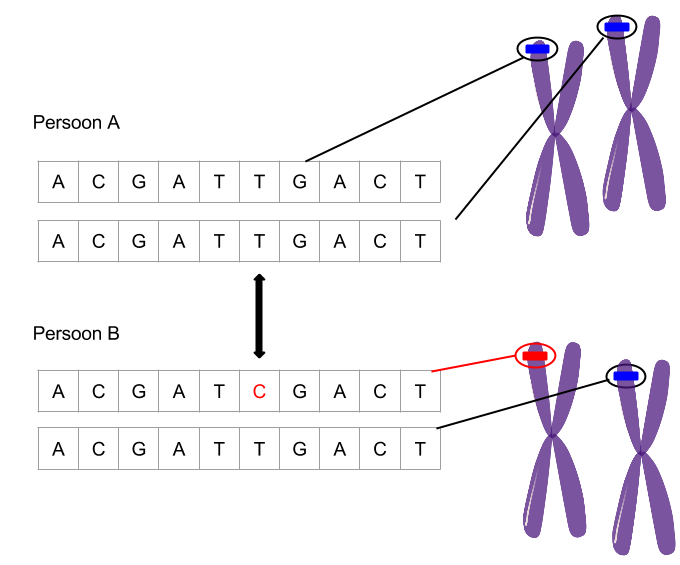
\includegraphics[width=\textwidth,keepaspectratio]{chrom_schema}
\caption{Een sequentie uit het DNA van 2 personen. De sequentie ligt op dezelfde locatie op het chromosoom bij beide personen, maar verschilt 1 nucleotide tussen de twee personen. De sequentie is dus een \textit{single nucleotide polymorphism} of \textit{variant}. Beide personen hebben ook twee allelen voor de variant. Persoon A is homozygoot, persoon B heterozygoot \cite{chrom_clipart}.}
\label{chrom_schema}
\end{figure}

\textbf{DNA sequencing} is het bepalen van de exacte sequentie van nucleotidebasen in een streng DNA. De vandaag meest gebruikte sequencingmethode genereert reads van 125 opeenvolgende nucleotiden, en miljarden reads tegelijkertijd. Om de segmenten horende in \'e\'en langer stuk DNA aan elkaar te kunnen linken, is het nodig vele overlappende segmenten te lezen, die vervolgens met elkaar gealigneerd worden. Elke nucleotide moet dus meerdere keren gelezen worden om een goede accuraatheid van het uiteindelijke resultaat te bekomen. De \textbf{depth} van een nucleotide, of bij uitbreiding een groter stuk DNA, is het aantal keren dat een nucleotide gelezen werd tijdens het sequencingproces. De \textbf{coverage} is de gemiddelde depth over de hele DNA-streng die gesequenced werd en dus een maat voor de resolutie en accuraatheid van het sequencingproces. De uiteindelijke sequencedata worden vaak opgeslagen in SAM-files (of BAM, het binaire equivalent) en het is op basis hiervan dat \textbf{variant calling} gebeurt: het bepalen welk genotype een proefpersoon precies heeft voor een variant.\\
De resultaten van het variant-callingproces worden opgeslagen in \textbf{VCF}-bestanden (Variant Call Format). Het VCF-formaat bevat naast meta-informatie een lijn voor elke geobserveerde variant, met daarin optioneel informatie over het genotype van \'e\'en of meerdere proefpersonen.\\
In onderzoek naar het DNA van proefpersonen is ook nog andere informatie van tel dan enkel hun genotypes: gegevens als het geslacht of fenotype van proefpersonen kunnen uiterst relevant zijn voor onderzoek naar bijvoorbeeld genetische ziektes. In experimenten die het DNA van meerdere proefpersonen analyseren, is het ook bijzonder interessant de onderlinge verwantschappen tussen de proefpersonen te kennen. Samen met de genotype-informatie is het dan mogelijk erfelijkheidspatronen in de genoomdata te bestuderen. Dergelijke gedetailleerde informatie over de proefpersonen zit echter niet in de VCF-files, maar kan gespecifieerd worden in zogenaamde pedigree-files (\textbf{PED}-files).\\\\

{\color{red}TODO: Voorbeeld vragen biologen}